\section{Rapport d'activité}

\subsection{Organisation du travail}


\subsection{Outils de développement}



\subsubsection{Communication}


\subsubsection{Unity}

Unity est un logiciel orienté pour le développement de jeux-vidéos intégrant un moteur physique 2D et 3D. Sa particularité réside dans la possibilité d'exporter l'application développée sur de nombreuses plateformes (Web, Android, iOS, Consoles..). Nous avons réalisé notre projet avec la version 5 du produit.


\begin{figure}[H]\centering
  \frame{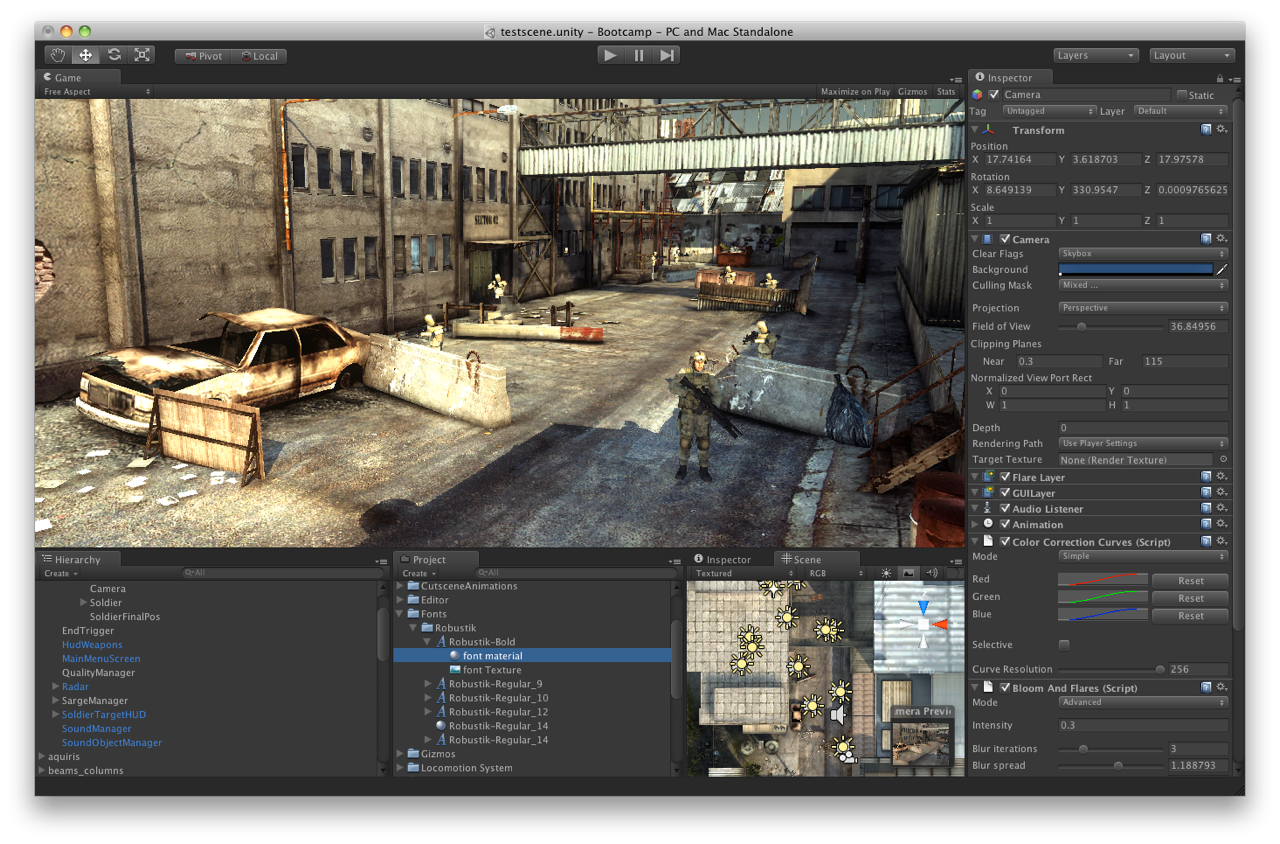
\includegraphics[scale=.28]{./img/unity-3D.png}}
  \caption{Interface de Unity}
  \label{unity}
\end{figure}

\paragraph{Pourquoi utiliser Unity ?}

Nous avons choisi de développer en utilisant Unity afin de pouvoir déployer notre jeu facilement sur les plateformes mobiles populaires (Android, iOS et Windows Phone), sans avoir à développer trois fois la même application dans un langage différent. De plus, l'utilisation du moteur d'Unity nous permet d'économiser le temps nécessaire à la création d'un moteur spécifique au projet, qui serait probablement mal optimisé. Enfin, la technologie Unity est de plus en plus populaire et de plus en plus de jeux voient le jour grâce à elle, nous avons donc profité du projet pour apprendre à l'utiliser.
 
\paragraph{Fonctionnalités d'Unity}
Dans notre projet, nous utilisons principalement Unity pour :
\begin{itemize}
\item Afficher des \textit{sprites}
\item Réaliser des animations
\item Jouer des sons
\item Créer l'interface utilisateur
\item Gérer les évènements clavier (ou tactiles)
\item Exporter sur de  multiples plateformes
\end{itemize}
Ce que nous n'utilisons pas avec Unity :
\begin{itemize}
\item Le moteur physique (gravité, collisions, squelettes...)
\item La 3D
\end{itemize}
Ainsi, il y a de nombreuses fonctionnalités nécessaires au développement de notre jeu qui ne sont pas gérées par Unity et que nous devons développer.
 
\paragraph{Principe de Unity}
Lorsqu'un nouveau projet Unity est démarré, il faut d'abord ajouter un ou plusieurs objets à une scène. Cet objet peut être de tout type : un solide, une lumière, une caméra, un son, des particules... Ensuite, il est possible de greffer un script à cet objet. Ce script peut être développé en Javascript ou en C\#. Il est possible d'exécuter des instructions lors de la création de l'objet, de sa destruction ou en encore à chaque rafraîchissement de l'écran. Chaque composantes de l'objet (taille, position, rendu...) sont accessibles et paramétrables directement dans le script. Enfin, les objets peuvent communiquer entre eux par le biais des scripts qui leur sont attachés.

\paragraph{Coût de Unity}
Unity possède deux types de versions : une version personnelle, et une version professionnelle. Les deux versions comportent les mêmes fonctionnalités, c'est à qu'il n'est pas forcément nécessaire d'acheter la version professionnelle pour développer un jeu-vidéo de grande envergure. Cependant, l'achat de la licence Unity est nécessaire lorsque l'entreprise réalise une revenu brut sur une année de plus de 100 000\$. L'achat de la version Unity Pro revient à 1500\$ (ou 75\$ par mois). Il est à noter qu'il est aussi nécessaire d'acheter les modules permettant d'exporter sous iOS ou Android, qui reviennent à 1500\$ chacun (ou 75\$ par mois). La version personnelle affichera néanmoins un \textit{splash-screen} au démarrage du jeu vidéo, et ce, sur n'importe quelle plateforme.

